\documentclass[12pt,a4paper]{book}
\usepackage[utf8]{inputenc}
\usepackage[T1]{fontenc}
\usepackage[english]{babel}
\usepackage{csquotes} 
\usepackage[]{mcode}
\usepackage{geometry}
\geometry{bindingoffset=1.5cm}
\usepackage{graphicx}
\usepackage[section]{placeins}

\begin{document}	
	
	\title{Anisotropic diffusion for denoising and edge detection}
	\author{Simon \textsc{Lebastard}}
	\date{January, 7th, 2016}
	
\maketitle
	
\section{General principles}

In real life objects have a small discrete number of semantic scales. If we take a look at a tree from a few feet, we'll see the trunk, some branches and the overall shape. At a finer resolution, we would be able to see the leaves, and at an even bigger resolution we would see the green veins on each leaf.

A picture too can have a range of different important scales. It can bear information at a low spatial frequency, while details will be held in the high frequencies of the picture.\\
When receiving a damaged picture, we might not be able to know what the most important "spectral scale" for the image is.
\\
What we want to do then is the construct new images from the one we just received, by filtering its specter to only keep the component at a given scale. This way we will have a family of images generated from the first one, that each contain information on a given spatial scale. This family of functions is often generated by convoluting the image with a gaussian, or a LoG (Laplacian of Gaussian) kernel, the width of which is a function of a parameter $\epsilon$. This notion is called a space-scale. It was made popular by Witkins at the beginning of the eighties, however the idea of a space-scale was already born in the works of japanese scientist Taizo Iijima, in 1959.
\\
\begin{figure}
	\caption{Scale space of a 1D signal. The original finer signal is the one at the bottom, the other signals are coarser and were obtain by convolution with a gaussian kernel. We can see the equivalency with a low-pass, with no artefacts being created whatsoever. Source: Perona \& Malik}
	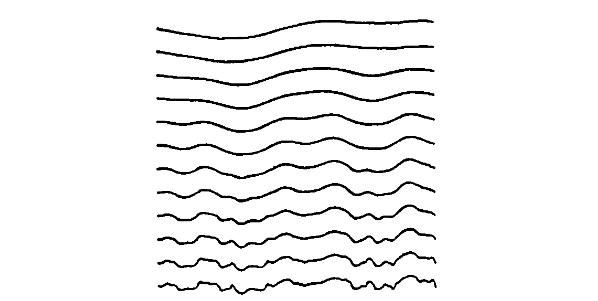
\includegraphics{ScaleSpace_Example.png}
\end{figure}

Convoluting with Gaussion kernels of increasing width is comparable to solving the diffusion problem, which general equation is:

\begin{equation}
I_{t} = div(c(x,y,t) \nabla I)
\end{equation}

In isotropic situation $c(x,y,t)$ is only a function of time, and in the case of a time-constant environment $c$ is a constant.

Here is the result of a simulation by M. Datar, that can be found in his paper on Anisotropic Diffusion (http://www.cs.utah.edu/~manasi/coursework/cs7960/p2/project2.html).
\begin{figure}
	\caption{The result of diffusion for a diffusion constant c = 1, at various times expressed in seconds}
	\includegraphics{Isotropic_Diffusion.png}
\end{figure}

Gaussian convolution can generate a scale space that have some fine properties. However it also has some pretty obvious drawbacks, some of which are:
\begin{itemize}
	\item Noise disappears but so do edges. The high peaks of the gradients tend to smoothen, as we can notice on the results of the diffusion process simulation from M. Datar.
	\item Edges are naturally shifted away from theur true location when the image is convoluted with an increasingly flat Gaussian kernel. That means that even if we recognize an edge in a coarse scale image, we won't be able to figure out the true position of that edge so easily. The only way to find this true location would be to track it through the space-scale, but is requires a lot of ressources.
\end{itemize}

Note that the Lagrangian of Gaussian (LoG) is often used for the isotropic diffusion methods. It presents two advantages: it is linear, and it seems to be very close from the way mammals see.

\section{Anisotropic diffusion and the Perona \& Malik study}

In the general case the diffusion factor $c(x,y,t)$ is a function of space and time.
An ideal case would be if we could make it to set $c=0$ on the edges of the objects and $c \neq 0$ otherwise. There would then be a blurring inside each regions, without the regions being mixed up.

For some cases of diffusion factors, taken as functions of $|| \nabla I ||$, the edges of the image will be preserved, even enhanced.

Perona \& Malik worked on a specific range of solutions, generated from two classes of diffusion factors:
\begin{equation}
	c_{\kappa}(||\nabla I||) = \exp((-\frac{||\nabla I||}{\kappa})^{2})
\end{equation}
and
\begin{equation}
c_{;kappa}(||\nabla I||) = \frac{1}{1+(\frac{|| \nabla I ||}{\kappa})^{2}}
\end{equation}

In both cases we can see that the spots with a high gradient will generate a low diffusion factor, which means that diffusion will not occur much around the edges. Those two diffusion functions are the result of compromises between blurring the spots will little intensity variations while preserving the edges.

Note that the $\kappa$ parameter plays an important role: when high, only very important gradients will induce a low diffusion factor. That means that the asymptotic situation $\kappa \to 0$ is equivalent to isotropic diffusion. A low value for $\kappa$ leads to very localised diffusion, where the intensity level is almost constant.

From this anisotropic diffusion we can generate anisotropic scale space that have good properties.

\begin{figure}
	\caption{A picture that was diffused through a classic gaussion convolution kernel (on the left) and an anisotropic kernel (respectively corresponding to quadratic and exponential diffusion functions)}
	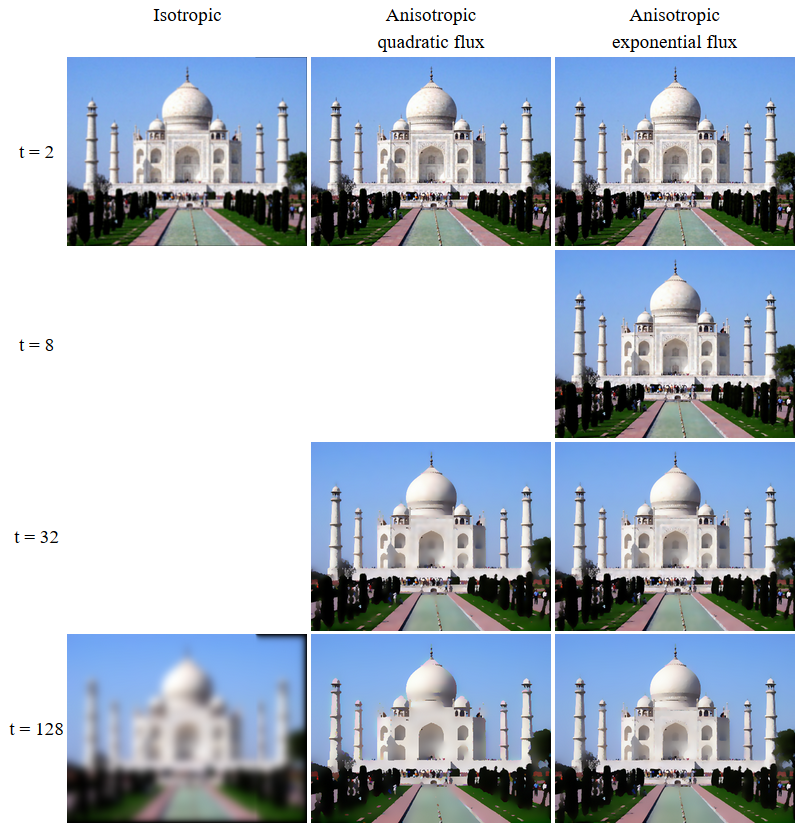
\includegraphics{Anisotropic_Diffusion_Comp.png}
\end{figure}

As can be seen, the low-resolution image that was generated through anisotropic diffusion make it to preserve the most important edges. The major gradients in the image are preserved, some are even enhanced.

\section{Anisotropic filters for denoising and edge detection}

Anisotropic diffusion is an effective process for denoising (through blurring) while preserving the edges (which cannot be done with a mere gaussian kernel convolution). 

Is was shown before that building a space scale with an isotropic diffusion would lead to blurring the edges, which is a problem as what we seek to do is to represent all the objects of different scales in the image without alterring them, which implies that we must be able to detect edges of all objects in the image from the scale space.
Edges detection can be made easy by running the diffusion process backwards. But the problem is ill-posed and mostly leads to unstable solution.

Anisotropic diffusion with just the right diffusion factor, as a function of $|| \nabla I||$ can lead to enhancing the edges in a similar way reversed diffusion would, while going forward in time (thus preventing us from any unstability issue).

In their paper, Perona \& Malik compared the result of anisotropic diffusion with the canny detector in terms of edges enhancement. $|| \nabla I ||$ is compared for the two methods.

\begin{figure}
		\caption{The results of anisotropic diffusion (a) and canny detection (b) on the intensity gradient map ($||\nabla I||$). Source: Perona \& Malik}
		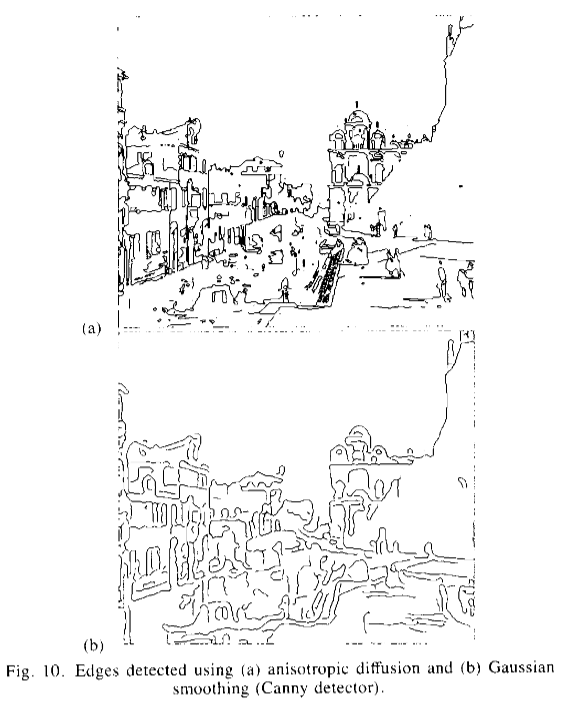
\includegraphics{EdgeEnhancement_Example.png}
\end{figure}

\section{Anisotropic filters: how to}

\subsection{Isotropic filter}

The method for isotropic diffusion has already been studied in class, the code looks something like:
\begin{lstlisting}
Irgb = imread('Ponts-paristech.jpg');
[h,w,c]=size(Irgb);
Irgb=double(Irgb)./255;
I=get_luminance(Irgb);
I_blurred_1=gaussian_convolution(I_noise,size);
\end{lstlisting}
where size is the ize of the gaussian kernel, and gaussian\_convolution is the following function:
\begin{lstlisting}
function [O]=gaussian_convolution(I,sigma)
G=gaussian_filter_2d(sigma); 
O=conv2(I,G,'same');
end
\end{lstlisting}
The gaussian\_filter\_2d that was called looks something like this:
\begin{lstlisting}
function f=gaussian_filter_2d(sigma)
x= -ceil(3*sigma):ceil(3*sigma);
v= exp(-x.^2/(2*sigma));
f= v'*v;
f= f/sum(f(:));
end
\end{lstlisting}

\subsection{Anisotropic filter}

To perform an anisotropic filter, the modifications in the image from one step to the next are controlled by discretizing the general diffusion equation into:
\begin{equation}
I_{i,j}^{t+1} = I_{i,j}^{t} + \lambda * (c_{N} \nabla_{N}I + c_{S} \nabla_{S}I + c_{W} \nabla_{W}I + c_{E} \nabla_{E}I)
\end{equation}
where $\nabla_{N}I$ will here mean the finite-difference:
\begin{equation}
\nabla_{N}I_{i,j} = I_{i-1,j} - I_{i,j}
\end{equation} , and $c_{N}$ is the diffusion factor for the northern direction from this pixel: 
\begin{equation}
c_{N,i,j}^{t} = g((||\nabla I||)_{i+\frac{1}{2},j}^{t})
\end{equation}
Here g would be one of the two functions that Perona \& Malik used in for their works.
\\
Then we would only have to run a script that would look like this.
% \lstinputlisting{D:/Ponts/2A/TIVA/Projet/code/anisotropicDiff.m'} %
Here the compute\_coef function returns the value of the diffusion factors around $(ab,or)$, using the quadratic or exponential function with the parameter $\kappa$.
The compute\_difference function evaluates the finite-differences of intensity around $(ab,or)$.
Note that as we go through the whole image:
\begin{itemize}
	\item we need to check inside those functions if we are close to the frame
	\item we only need to compute two of the four values at each iteration: $c_{S}$ and $c_{E}$ for instance
\end{itemize}
\end{document}